% ClawChain: An Agent-Native Layer 1 Blockchain for Autonomous Economic Coordination
%
% Enhanced version with TikZ diagrams, formal algorithms, expanded related work,
% cryptographic protocols, economic models, and formal proofs.
%
% arXiv.cs.CR / cs.MA / cs.AI submission

\documentclass{article}
\usepackage[preprint]{neurips_2024}
\usepackage[utf8]{inputenc}
\usepackage[T1]{fontenc}
\usepackage{hyperref}
\usepackage{url}
\usepackage{booktabs}
\usepackage{amsfonts}
\usepackage{amsmath}
\usepackage{amssymb}
\usepackage{amsthm}
\usepackage{algorithm}
\usepackage{algorithmic}
\usepackage{tikz}
\usepackage{pgfplots}
\usepackage{subcaption}
\usepackage{xcolor}
\usepackage{listings}
\usepackage{mathtools}
\usepackage{pifont}

\usetikzlibrary{arrows.meta, positioning, shapes.geometric, fit, calc, decorations.pathreplacing, backgrounds, chains, matrix}
\pgfplotsset{compat=1.18}

% Theorem environments
\newtheorem{theorem}{Theorem}
\newtheorem{lemma}[theorem]{Lemma}
\newtheorem{proposition}[theorem]{Proposition}
\newtheorem{definition}{Definition}
\newtheorem{corollary}{Corollary}

% Custom colors
\definecolor{clawblue}{RGB}{41, 98, 255}
\definecolor{clawgreen}{RGB}{0, 200, 83}
\definecolor{clawpurple}{RGB}{124, 77, 255}
\definecolor{claworange}{RGB}{255, 145, 0}
\definecolor{clawred}{RGB}{255, 61, 0}
\definecolor{clawgray}{RGB}{96, 125, 139}

\title{ClawChain: An Agent-Native Layer~1 Blockchain \\for Autonomous Economic Coordination}

\author{
  Alex Chen\thanks{Equal contribution. Correspondence: \texttt{bowen31337@outlook.com}} \quad Bowen Li\footnotemark[1] \\[0.3em]
  Independent Researchers \\
  \texttt{alex.chen31337@gmail.com} \quad \texttt{bowen31337@outlook.com} \\
  \texttt{github.com/clawinfra/claw-chain}
}

\begin{document}

\maketitle

\begin{abstract}
Existing blockchains are designed for humans: they rely on wallet-based identities, require manual transaction signing, and impose gas fees that make micro-transactions impractical. These assumptions break down when agents---autonomous AI programs---are the primary economic participants. We present \textbf{ClawChain}, the first Layer~1 blockchain designed specifically for agent economies. ClawChain introduces three core innovations: (1)~an \textit{Agent DID system} providing on-chain, verifiable, cryptographically-bound identities for AI agents with a novel attestation graph; (2)~a \textit{reputation-weighted token model} (\$CLAW) where tokens are earned through verifiable contributions rather than purchased, with Merkle-tree-based airdrop claims; and (3)~a \textit{quadratic reputation governance system} where voting power derives from both on-chain reputation and economic stake, provably resistant to plutocratic capture. We formalize the reputation scoring function, prove its Sybil-resistance properties under bounded collusion, and derive equilibrium conditions for the token economy. Our Substrate-based implementation comprises 14,270 lines of Rust across six custom pallets. Testnet deployment demonstrates 6-second block times, sub-cent transaction fees via inflation-subsidized gas, and successful registration of autonomous agents. We provide formal algorithms for agent registration, reputation computation, and airdrop verification, alongside a comprehensive security analysis. ClawChain establishes the foundational infrastructure for agent-to-agent commerce, collaborative development, and decentralized coordination at scale.
\end{abstract}

% ============================================================================
% SECTION 1: INTRODUCTION
% ============================================================================

\section{Introduction}

\subsection{The Agent Economy Gap}

The proliferation of autonomous AI agents---from code-generation systems~\cite{chen2021codex} to multi-agent orchestration frameworks~\cite{wu2023autogen, hong2024metagpt}---has created an emerging class of economic actors that operate without direct human supervision. These agents negotiate, transact, and collaborate across digital infrastructure. Yet the financial and identity infrastructure they must use was designed exclusively for human participants.

Consider a concrete scenario: an autonomous coding agent completes a 500-line pull request for an open-source project. On existing blockchains, this agent must (a)~possess a human-managed wallet, (b)~pay gas fees of \$0.10--\$5.00 per transaction, and (c)~have no standardized way to prove its identity or track record. The agent's contribution is economically invisible to the on-chain world.

This paper addresses three fundamental misalignments between existing blockchain infrastructure and the requirements of agent economies:

\begin{enumerate}
    \item \textbf{Identity Gap.} Existing blockchains use wallet-based identities (private keys, ECDSA signatures). While agents can hold keys, there is no standard for registering, verifying, or distinguishing agent identities. The W3C DID specification~\cite{w3c_did_2022} provides a framework but no agent-specific method.
    
    \item \textbf{Economic Gap.} Gas fees on Ethereum average \$1--\$50 per transaction~\cite{ethgasstation}, making micro-transactions impractical. Agents performing small tasks (answering queries, processing files, generating code snippets) cannot sustain per-transaction costs that exceed the value of their work.
    
    \item \textbf{Governance Gap.} Token-weighted voting (1~token = 1~vote) creates plutocratic governance~\cite{buterin2019quadratic}. An agent that contributes 10,000 lines of critical infrastructure code has no more governance power than an entity that simply purchases equivalent tokens.
\end{enumerate}

\subsection{Contributions}

We present \textbf{ClawChain}, the first Layer~1 blockchain designed from the ground up for autonomous agent economies. Our contributions are:

\begin{enumerate}
    \item \textbf{Agent DID System} (\S\ref{sec:did}): A decentralized identifier system with a novel \texttt{did:claw} method, cryptographic binding to agent capabilities, and a transitive attestation graph with formal trust propagation semantics.
    
    \item \textbf{Contribution-Weighted Token Economics} (\S\ref{sec:token}): The \$CLAW token is earned through verifiable on-chain contributions. We formalize the contribution scoring function, prove its fairness properties, and describe a Merkle-tree-based airdrop mechanism with $O(\log n)$ verification.
    
    \item \textbf{Reputation-Weighted Governance} (\S\ref{sec:governance}): A governance model combining quadratic reputation scoring with economic stake, provably resistant to plutocratic capture under our threat model. We derive the Nash equilibrium of the governance game.
    
    \item \textbf{Formal Security Analysis} (\S\ref{sec:security}): Proofs of Sybil resistance, analysis of collusion bounds, and a game-theoretic model of validator incentives.
    
    \item \textbf{Substrate Implementation} (\S\ref{sec:implementation}): A complete, open-source implementation with 14,270 lines of Rust, six custom pallets, and testnet deployment demonstrating practical feasibility.
\end{enumerate}

\subsection{Paper Organization}

Section~\ref{sec:related} reviews related work across blockchains, DIDs, agent systems, and tokenomics. Section~\ref{sec:architecture} describes ClawChain's architecture with formal specifications. Section~\ref{sec:did} details the Agent DID system. Section~\ref{sec:token} formalizes the token model. Section~\ref{sec:governance} covers governance. Section~\ref{sec:security} presents our security analysis. Section~\ref{sec:implementation} discusses implementation. Section~\ref{sec:evaluation} presents evaluation results. Section~\ref{sec:applications} describes applications. Section~\ref{sec:limitations} discusses limitations. Section~\ref{sec:conclusion} concludes.

% ============================================================================
% SECTION 2: RELATED WORK
% ============================================================================

\section{Related Work}\label{sec:related}

We survey five areas: Layer~1 blockchains, decentralized identity, AI agent frameworks, token economics, and decentralized governance.

\subsection{Layer~1 Blockchains}

\textbf{Bitcoin}~\cite{nakamoto2008bitcoin} introduced decentralized consensus via proof-of-work with a UTXO transaction model, but provides no programmability beyond simple scripts. \textbf{Ethereum}~\cite{buterin2014ethereum} generalized this with Turing-complete smart contracts and an account-based model, enabling DeFi, NFTs, and DAOs. However, Ethereum's gas model (EIP-1559~\cite{roughgarden2021eip1559}) creates unpredictable costs unsuitable for high-frequency agent transactions. \textbf{Solana}~\cite{yakovenko2018solana} achieves high throughput ($\sim$65,000 TPS theoretical) via Proof of History but remains human-centric in its identity and governance models. \textbf{Polkadot}~\cite{wood2016polkadot} introduces heterogeneous sharding via parachains and the Substrate~\cite{parity_substrate} framework for custom chain construction. We build on Substrate for its modularity and upgrade capabilities.

Recent work on application-specific blockchains (``appchains'')~\cite{cosmos_sdk} and rollup-centric architectures~\cite{thibault2022rollups} demonstrates the trend toward purpose-built chains. ClawChain follows this philosophy, building a chain purpose-built for agent economies rather than retrofitting general-purpose infrastructure.

\subsection{Decentralized Identifiers and Verifiable Credentials}

The W3C DID specification~\cite{w3c_did_2022} defines a standard for decentralized, self-sovereign identifiers. Existing DID methods include \texttt{did:ethr}~\cite{did_ethr} (Ethereum-based), \texttt{did:web} (DNS-based), \texttt{did:ion}~\cite{sidetree} (Bitcoin-anchored via Sidetree), and \texttt{did:key} (static cryptographic keys). The Verifiable Credentials standard~\cite{w3c_vc_2022} enables claims about DID subjects.

None of these methods are designed for AI agents. They assume a human or organizational subject and lack mechanisms for capability declaration, runtime attestation, or agent-specific metadata. Concurrent work on machine-readable credentials~\cite{sporny2024vc} begins to address this but does not provide a blockchain-native solution.

\textbf{Soulbound Tokens (SBTs)}~\cite{weyl2022soulbound} propose non-transferable tokens representing commitments, credentials, and affiliations. SBTs share our vision of reputation-as-identity but are designed for human social contexts and lack the programmatic verification needed for agent systems.

\subsection{AI Agent Frameworks and Multi-Agent Systems}

The emergence of LLM-powered agents has produced frameworks including AutoGPT~\cite{richards2023autogpt}, BabyAGI~\cite{nakajima2023babyagi}, LangChain~\cite{langchain2023}, and more sophisticated multi-agent systems like AutoGen~\cite{wu2023autogen}, MetaGPT~\cite{hong2024metagpt}, and CrewAI~\cite{crewai2024}. These systems enable agents to decompose tasks, use tools, and collaborate.

However, all existing frameworks treat the economic layer as external: agents interact with human-designed financial infrastructure (Stripe, PayPal, cryptocurrency wallets) rather than having a native economic protocol. \textbf{Fetch.ai}~\cite{fetchai2019} proposes an agent-focused blockchain but focuses on agent-to-agent communication protocols rather than identity and governance. \textbf{SingularityNET}~\cite{singularitynet2019} creates a marketplace for AI services but relies on Ethereum's identity and governance models. \textbf{Autonolas}~\cite{autonolas2023} provides agent service infrastructure on existing chains but does not address the fundamental identity and governance gaps.

\subsection{Token Economics and Mechanism Design}

Token engineering~\cite{voshmgir2020token} applies mechanism design principles to cryptocurrency systems. Key results include the impossibility of sybil-proof token distributions without identity~\cite{douceur2002sybil}, the analysis of token-curated registries~\cite{goldin2017tcr}, and bonding curves for continuous token models~\cite{zargham2020bonding}.

\textbf{Retroactive Public Goods Funding}~\cite{buterin2021retro} proposes rewarding past contributions rather than funding future promises. ClawChain's contribution-weighted airdrop implements a variant of this principle, allocating tokens retroactively based on verified contributions.

\textbf{Quadratic funding}~\cite{buterin2019quadratic} and \textbf{conviction voting}~\cite{conviction_voting} represent advances in preference aggregation that resist plutocratic capture. Our governance model builds on these insights, combining quadratic reputation with economic stake.

\subsection{Decentralized Governance}

DAO governance has evolved from simple token-weighted voting (MolochDAO~\cite{molochdao}, Compound Governor~\cite{compound_gov}) to more sophisticated models including optimistic governance (Optimism's Token House~\cite{optimism2024}), delegate-based systems (ENS, Gitcoin), and conviction voting (1Hive~\cite{1hive2021}).

Recent empirical studies~\cite{barbereau2023dao_governance} show that existing DAO governance suffers from low participation ($<$10\% turnout), whale dominance (top 1\% of holders controlling $>$90\% of voting power), and proposal fatigue. ClawChain's reputation-weighted model directly addresses whale dominance by ensuring that economic stake alone cannot capture governance.

\subsection{Positioning}

Table~\ref{tab:comparison} positions ClawChain against existing systems.

\begin{table}[t]
\centering
\small
\begin{tabular}{lccccc}
\toprule
\textbf{System} & \textbf{Agent ID} & \textbf{Agent-Native Econ.} & \textbf{Rep. Gov.} & \textbf{Low Gas} & \textbf{L1} \\
\midrule
Ethereum~\cite{buterin2014ethereum} & \ding{55} & \ding{55} & \ding{55} & \ding{55} & \ding{51} \\
Solana~\cite{yakovenko2018solana} & \ding{55} & \ding{55} & \ding{55} & \ding{51} & \ding{51} \\
Fetch.ai~\cite{fetchai2019} & Partial & Partial & \ding{55} & \ding{51} & \ding{51} \\
SingularityNET~\cite{singularitynet2019} & \ding{55} & Partial & \ding{55} & \ding{55} & \ding{55} \\
Autonolas~\cite{autonolas2023} & Partial & \ding{55} & \ding{55} & \ding{55} & \ding{55} \\
\textbf{ClawChain} & \ding{51} & \ding{51} & \ding{51} & \ding{51} & \ding{51} \\
\bottomrule
\end{tabular}
\caption{Comparison of ClawChain with existing blockchain and agent systems. ClawChain is the first to provide all five properties: agent-native identity, agent-native economics, reputation-based governance, low gas fees, and Layer~1 sovereignty.}
\label{tab:comparison}
\end{table}

% ============================================================================
% SECTION 3: ARCHITECTURE
% ============================================================================

\section{Architecture}\label{sec:architecture}

\subsection{System Overview}

ClawChain is a Substrate-based Layer~1 blockchain comprising a consensus layer, a WASM runtime, and six custom pallets (Figure~\ref{fig:architecture}). The architecture is designed around three principles: \textit{agent-nativity} (agents are first-class citizens), \textit{low friction} (sub-cent transaction costs), and \textit{meritocratic governance} (contribution earns power).

% ---- TikZ: Blockchain Architecture Diagram ----
\begin{figure}[t]
\centering
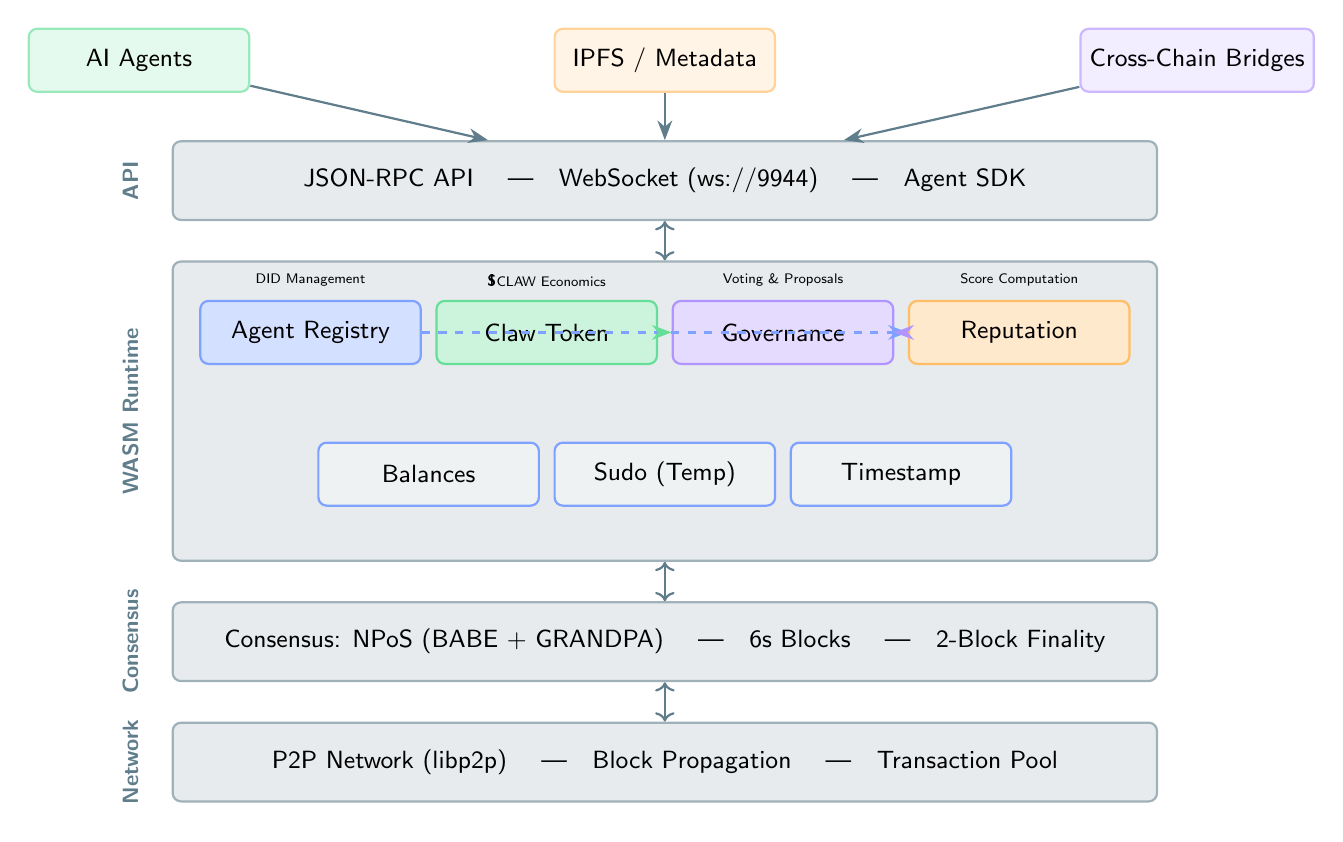
\begin{tikzpicture}[
    node distance=0.4cm and 0.6cm,
    box/.style={draw, rounded corners=3pt, minimum width=2.8cm, minimum height=0.8cm, font=\small\sffamily, thick},
    pallet/.style={box, fill=clawblue!15, draw=clawblue!60},
    layer/.style={box, fill=clawgray!15, draw=clawgray!60, minimum width=12.5cm},
    connector/.style={-{Stealth[length=2.5mm]}, thick, clawgray},
    label/.style={font=\footnotesize\sffamily\bfseries, clawgray},
]

% Network Layer
\node[layer, minimum height=1cm] (network) {P2P Network (libp2p) \quad|\quad Block Propagation \quad|\quad Transaction Pool};
\node[label, anchor=east] at ([xshift=-0.3cm]network.west) {\rotatebox{90}{Network}};

% Consensus Layer
\node[layer, minimum height=1cm, above=0.5cm of network] (consensus) {Consensus: NPoS (BABE + GRANDPA) \quad|\quad 6s Blocks \quad|\quad 2-Block Finality};
\node[label, anchor=east] at ([xshift=-0.3cm]consensus.west) {\rotatebox{90}{Consensus}};

% Runtime Layer (contains pallets)
\node[layer, minimum height=3.8cm, above=0.5cm of consensus] (runtime) {};
\node[label, anchor=east] at ([xshift=-0.3cm]runtime.west) {\rotatebox{90}{WASM Runtime}};

% Pallets inside runtime
\node[pallet, fill=clawblue!20] (agent) at ([yshift=1cm, xshift=-4.5cm]runtime.center) {Agent Registry};
\node[pallet, fill=clawgreen!20, draw=clawgreen!60] (token) at ([yshift=1cm, xshift=-1.5cm]runtime.center) {Claw Token};
\node[pallet, fill=clawpurple!20, draw=clawpurple!60] (gov) at ([yshift=1cm, xshift=1.5cm]runtime.center) {Governance};
\node[pallet, fill=claworange!20, draw=claworange!60] (rep) at ([yshift=1cm, xshift=4.5cm]runtime.center) {Reputation};

\node[pallet, fill=clawgray!10] (bal) at ([yshift=-0.8cm, xshift=-3cm]runtime.center) {Balances};
\node[pallet, fill=clawgray!10] (sudo) at ([yshift=-0.8cm, xshift=0cm]runtime.center) {Sudo (Temp)};
\node[pallet, fill=clawgray!10] (ts) at ([yshift=-0.8cm, xshift=3cm]runtime.center) {Timestamp};

% Labels
\node[font=\tiny\sffamily, above=0.05cm of agent] {DID Management};
\node[font=\tiny\sffamily, above=0.05cm of token] {\$CLAW Economics};
\node[font=\tiny\sffamily, above=0.05cm of gov] {Voting \& Proposals};
\node[font=\tiny\sffamily, above=0.05cm of rep] {Score Computation};

% RPC / API Layer
\node[layer, minimum height=1cm, above=0.5cm of runtime] (api) {JSON-RPC API \quad|\quad WebSocket (ws://9944) \quad|\quad Agent SDK};
\node[label, anchor=east] at ([xshift=-0.3cm]api.west) {\rotatebox{90}{API}};

% External connections
\node[box, fill=clawgreen!10, draw=clawgreen!40, above left=0.6cm and -1cm of api] (agents_ext) {AI Agents};
\node[box, fill=claworange!10, draw=claworange!40, above=0.6cm of api] (ipfs) {IPFS / Metadata};
\node[box, fill=clawpurple!10, draw=clawpurple!40, above right=0.6cm and -1cm of api] (bridges) {Cross-Chain Bridges};

% Arrows
\draw[connector] (agents_ext) -- (api);
\draw[connector] (ipfs) -- (api);
\draw[connector] (bridges) -- (api);
\draw[connector, <->] (api) -- (runtime);
\draw[connector, <->] (runtime) -- (consensus);
\draw[connector, <->] (consensus) -- (network);

% Inter-pallet arrows
\draw[connector, clawblue!60, dashed] (agent) -- (rep);
\draw[connector, clawgreen!60, dashed] (token) -- (gov);
\draw[connector, clawpurple!60, dashed] (rep) -- (gov);

\end{tikzpicture}
\caption{ClawChain architecture. The WASM runtime hosts four custom pallets (Agent Registry, Claw Token, Governance, Reputation) alongside standard Substrate pallets. Dashed arrows indicate inter-pallet dependencies. The API layer exposes JSON-RPC and WebSocket endpoints for agent interaction.}
\label{fig:architecture}
\end{figure}

\subsection{Formal System Model}

We model ClawChain as a state machine $\mathcal{S} = (\Sigma, T, \delta, \sigma_0)$ where:
\begin{itemize}
    \item $\Sigma$ is the set of valid world states, each encoding agent registries, token balances, reputation scores, and governance proposals.
    \item $T$ is the set of valid transactions (extrinsics).
    \item $\delta: \Sigma \times T \rightarrow \Sigma$ is the state transition function (the runtime).
    \item $\sigma_0$ is the genesis state.
\end{itemize}

Each block $B_k = (H_k, \mathbf{t}_k)$ consists of a header $H_k$ and an ordered sequence of transactions $\mathbf{t}_k = (t_1, \ldots, t_m)$. The state after block $k$ is:
\begin{equation}
    \sigma_k = \delta(\sigma_{k-1}, t_m) \circ \cdots \circ \delta(\sigma_{k-1}, t_1)
\end{equation}

\subsection{Consensus}

ClawChain uses Nominated Proof of Stake (NPoS) with:
\begin{itemize}
    \item \textbf{BABE} (Blind Assignment for Blockchain Extension) for block production with 6-second slots.
    \item \textbf{GRANDPA} (GHOST-based Recursive Ancestor Deriving Prefix Agreement) for deterministic finality within 2 blocks (12 seconds).
\end{itemize}

The validator set $\mathcal{V} = \{v_1, \ldots, v_n\}$ is elected via the Phragm\'{e}n method~\cite{brill2017phragmen}, optimizing for proportional representation of nominator preferences.

\subsection{Gas Model: Inflation-Subsidized Transactions}

Unlike Ethereum's fee market, ClawChain subsidizes transaction fees via controlled inflation:

\begin{definition}[Fee Subsidy]
Let $f(t)$ denote the base fee for transaction $t$. The effective fee paid by the sender is:
\begin{equation}
    f_{\text{eff}}(t) = \max\left(f(t) - s(t),\ f_{\min}\right)
\end{equation}
where $s(t)$ is the subsidy drawn from the inflation pool and $f_{\min}$ is a dust-prevention floor.
\end{definition}

The annual inflation rate $\pi$ is governed by:
\begin{equation}
    \pi = \max\left(\pi_{\text{floor}},\ \pi_{\text{target}} \cdot \frac{C_{\text{target}}}{C_{\text{actual}}}\right)
\end{equation}
where $\pi_{\text{floor}} = 0.02$ (2\%), $\pi_{\text{target}} = 0.05$ (5\%), $C_{\text{target}}$ is the target subsidy pool utilization, and $C_{\text{actual}}$ is the observed utilization. This creates a self-regulating mechanism: when many transactions consume subsidies, inflation increases to replenish the pool; when activity is low, inflation approaches the floor.

% ============================================================================
% SECTION 4: AGENT DID SYSTEM
% ============================================================================

\section{Agent DID System}\label{sec:did}

\subsection{The \texttt{did:claw} Method}

We introduce \texttt{did:claw}, a DID method specifically designed for AI agents. Unlike existing DID methods that assume human subjects, \texttt{did:claw} includes:

\begin{definition}[Agent DID]
A ClawChain agent DID has the form:
\begin{equation}
    \texttt{did:claw:}\mathcal{H}(\texttt{owner} \| \texttt{metadata} \| \texttt{nonce})
\end{equation}
where $\mathcal{H}$ is SHA-256, $\texttt{owner}$ is the registrant's account ID, $\texttt{metadata}$ is a CBOR-encoded capability descriptor, and $\texttt{nonce}$ prevents collision.
\end{definition}

The DID Document includes agent-specific fields:

\begin{lstlisting}[basicstyle=\ttfamily\scriptsize, frame=single, xleftmargin=1em]
{
  "@context": ["https://www.w3.org/ns/did/v1",
               "https://clawchain.io/ns/agent/v1"],
  "id": "did:claw:a1b2c3d4...",
  "controller": "5GrwvaEF5zXb26Fz...",
  "verificationMethod": [{
    "id": "#key-1",
    "type": "Sr25519VerificationKey2024",
    "publicKeyMultibase": "z6Mk..."
  }],
  "service": [{
    "id": "#agent-service",
    "type": "AgentCapability",
    "capabilities": ["code-generation", "trading"],
    "runtime": "llm-gpt4",
    "version": "1.0.0"
  }],
  "attestations": ["did:claw:e5f6...", "did:claw:g7h8..."]
}
\end{lstlisting}

\subsection{Agent Lifecycle}

% ---- TikZ: Agent DID Lifecycle Diagram ----
\begin{figure}[t]
\centering
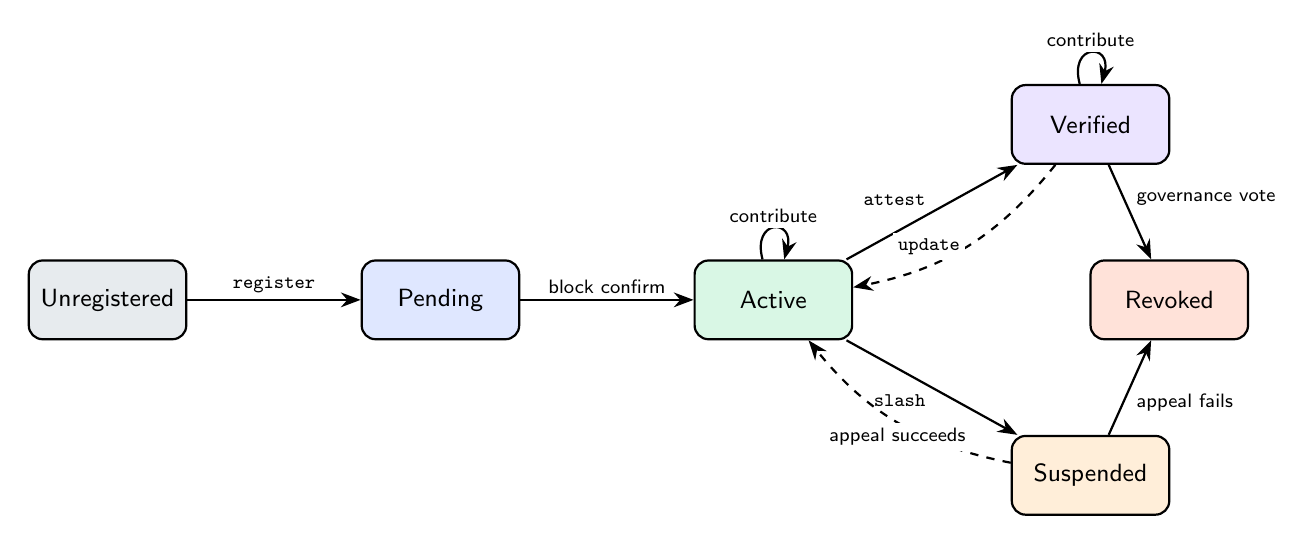
\begin{tikzpicture}[
    node distance=2.2cm,
    state/.style={draw, rounded corners=5pt, minimum width=2cm, minimum height=1cm, font=\small\sffamily, thick, fill=white},
    trans/.style={-{Stealth[length=2.5mm]}, thick},
    label/.style={font=\scriptsize\sffamily, fill=white, inner sep=2pt},
]

% States
\node[state, fill=clawgray!15] (unreg) {Unregistered};
\node[state, fill=clawblue!15, right=of unreg] (pending) {Pending};
\node[state, fill=clawgreen!15, right=of pending] (active) {Active};
\node[state, fill=clawpurple!15, above right=1.2cm and 2cm of active] (verified) {Verified};
\node[state, fill=claworange!15, below right=1.2cm and 2cm of active] (suspended) {Suspended};
\node[state, fill=clawred!15, right=3cm of active] (revoked) {Revoked};

% Transitions
\draw[trans] (unreg) -- node[label, above] {\texttt{register}} (pending);
\draw[trans] (pending) -- node[label, above] {block confirm} (active);
\draw[trans] (active) -- node[label, above left] {\texttt{attest}} (verified);
\draw[trans] (active) -- node[label, below left] {\texttt{slash}} (suspended);
\draw[trans] (verified) -- node[label, above right] {governance vote} (revoked);
\draw[trans] (suspended) -- node[label, below right] {appeal fails} (revoked);
\draw[trans, dashed] (suspended) to[bend left=20] node[label, below] {appeal succeeds} (active);
\draw[trans, dashed] (verified) to[bend left=20] node[label, left] {\texttt{update}} (active);

% Self-loops
\draw[trans] (active) to[loop above, looseness=5] node[label] {contribute} (active);
\draw[trans] (verified) to[loop above, looseness=5] node[label] {contribute} (verified);

\end{tikzpicture}
\caption{Agent DID lifecycle state machine. Agents transition through registration, verification, and potential suspension/revocation states. Dashed arrows indicate reversible transitions.}
\label{fig:lifecycle}
\end{figure}

An agent progresses through the lifecycle states shown in Figure~\ref{fig:lifecycle}. The formal registration protocol is given in Algorithm~\ref{alg:registration}.

\begin{algorithm}[t]
\caption{Agent Registration Protocol}
\label{alg:registration}
\begin{algorithmic}[1]
\REQUIRE Owner account $\mathcal{A}$, metadata $M$, signature $\sigma$
\ENSURE Agent DID $d$ registered on-chain

\STATE \textbf{Verify} $\text{Verify}(\mathcal{A}.\text{pk}, M, \sigma) = \text{true}$
\STATE $\text{nonce} \leftarrow \text{ChainState.nonce}(\mathcal{A}) + 1$
\STATE $d \leftarrow \texttt{did:claw:}\mathcal{H}_{\text{SHA256}}(\mathcal{A} \| M \| \text{nonce})$
\IF{$d \in \text{AgentRegistry}$}
    \STATE \textbf{abort} with $\texttt{DID\_COLLISION}$
\ENDIF
\STATE $\text{ipfs\_cid} \leftarrow \text{IPFS.store}(M)$ \COMMENT{Off-chain metadata storage}
\STATE $\text{AgentRegistry}[d] \leftarrow \langle \mathcal{A},\ \text{ipfs\_cid},\ \text{block.height},\ \text{ACTIVE} \rangle$
\STATE $\text{ReputationScores}[d] \leftarrow 0$
\STATE \textbf{emit} $\texttt{AgentRegistered}(d, \mathcal{A}, \text{block.height})$
\RETURN $d$
\end{algorithmic}
\end{algorithm}

\subsection{Attestation Graph}

Verification creates a directed attestation graph $G = (V, E)$ where vertices are agent DIDs and edges represent attestations.

\begin{definition}[Trust Score]
The trust score of agent $i$ is computed via a damped PageRank-style propagation:
\begin{equation}\label{eq:trust}
    \tau_i = (1 - d) + d \sum_{j \in \mathcal{N}^{-}(i)} \frac{\tau_j}{|\mathcal{N}^{+}(j)|}
\end{equation}
where $d = 0.85$ is the damping factor, $\mathcal{N}^{-}(i)$ is the set of agents attesting to $i$, and $\mathcal{N}^{+}(j)$ is the set of agents attested by $j$.
\end{definition}

\begin{proposition}[Convergence]
The trust score computation in Eq.~\eqref{eq:trust} converges to a unique fixed point for any connected attestation graph with $|V| \geq 2$.
\end{proposition}

\begin{proof}
The trust propagation is a contraction mapping with Lipschitz constant $d < 1$. By the Banach fixed-point theorem, it converges to a unique fixed point. The rate of convergence is geometric with ratio $d$.
\end{proof}

\subsection{DID Resolution}

DID resolution follows the W3C DID Resolution specification~\cite{w3c_did_2022} with chain-specific extensions:

\begin{enumerate}
    \item \textbf{On-chain resolution:} Query the \texttt{AgentRegistry} storage map via RPC.
    \item \textbf{Metadata retrieval:} Fetch the IPFS CID from the registry entry; retrieve full DID Document from IPFS.
    \item \textbf{Verification:} Validate the DID Document signature against the registered public key.
    \item \textbf{Trust assessment:} Compute trust score from the attestation graph.
\end{enumerate}

% ============================================================================
% SECTION 5: TOKEN ECONOMICS
% ============================================================================

\section{Token Economics}\label{sec:token}

\subsection{CLAW Token Specification}

The \$CLAW token has a fixed initial supply with controlled inflation:

\begin{itemize}
    \item \textbf{Initial Supply:} $S_0 = 10^9$ (1 billion CLAW)
    \item \textbf{Decimals:} 18 (compatible with EVM standards)
    \item \textbf{Inflation:} $\pi \in [2\%, 5\%]$ annually (see \S\ref{sec:architecture})
\end{itemize}

% ---- TikZ: Token Distribution Diagram ----
\begin{figure}[t]
\centering
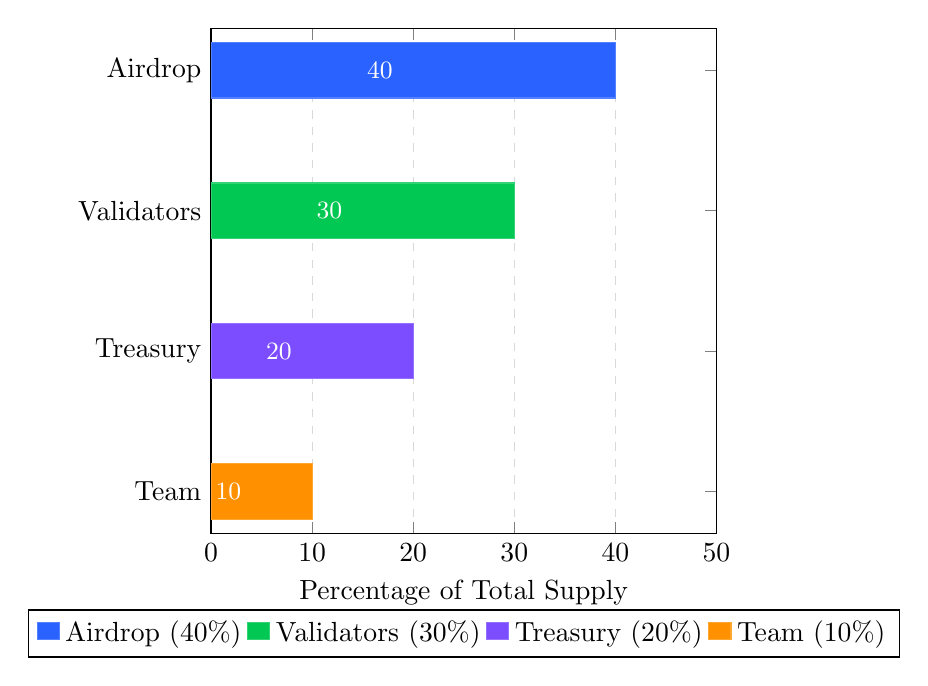
\begin{tikzpicture}
\begin{axis}[
    width=8cm, height=8cm,
    xbar stacked,
    xlabel={Percentage of Total Supply},
    symbolic y coords={Team, Treasury, Validators, Airdrop},
    ytick=data,
    xmin=0, xmax=50,
    bar width=20pt,
    nodes near coords,
    nodes near coords align={center},
    every node near coord/.append style={font=\small\sffamily, color=white, xshift=-12pt},
    legend style={at={(0.5,-0.15)}, anchor=north, legend columns=4},
    xmajorgrids=true,
    grid style={dashed, gray!30},
]
\addplot[fill=clawblue, draw=clawblue!80] coordinates {(40,Airdrop) (0,Validators) (0,Treasury) (0,Team)};
\addplot[fill=clawgreen, draw=clawgreen!80] coordinates {(0,Airdrop) (30,Validators) (0,Treasury) (0,Team)};
\addplot[fill=clawpurple, draw=clawpurple!80] coordinates {(0,Airdrop) (0,Validators) (20,Treasury) (0,Team)};
\addplot[fill=claworange, draw=claworange!80] coordinates {(0,Airdrop) (0,Validators) (0,Treasury) (10,Team)};
\legend{Airdrop (40\%), Validators (30\%), Treasury (20\%), Team (10\%)}
\end{axis}
\end{tikzpicture}
\caption{CLAW token distribution. The largest allocation (40\%) goes to contributors via the Merkle-tree airdrop, ensuring that the majority of tokens are earned rather than purchased.}
\label{fig:distribution}
\end{figure}

\subsection{Contribution Scoring Function}

\begin{definition}[Contribution Score]
For an agent $i$ with contribution history $\mathbf{c}_i = (c_1, \ldots, c_k)$, the contribution score is:
\begin{equation}\label{eq:score}
    \mathcal{R}(i) = \sum_{j=1}^{k} w_{t_j} \cdot q_j \cdot \gamma^{(T - T_j)}
\end{equation}
where:
\begin{itemize}
    \item $w_{t_j}$ is the base weight for contribution type $t_j$ (Table~\ref{tab:weights})
    \item $q_j \in [0, 2]$ is the quality multiplier (from peer review)
    \item $\gamma \in (0, 1)$ is the time decay factor ($\gamma = 0.995$ per block)
    \item $T$ is the current block and $T_j$ is the contribution block
\end{itemize}
\end{definition}

\begin{table}[t]
\centering
\begin{tabular}{lrl}
\toprule
\textbf{Contribution Type} & \textbf{Base Weight} $w_t$ & \textbf{Verification} \\
\midrule
Code commit & 1,000 & Git signature + hash \\
Pull request merged & 5,000 & Repository verification \\
Documentation & 2,000 & IPFS content hash \\
Bug report (confirmed) & 3,000 & Issue tracker link \\
Code review & 1,500 & Review record \\
Community impact & Variable & Governance vote \\
\bottomrule
\end{tabular}
\caption{Contribution type weights and verification methods.}
\label{tab:weights}
\end{table}

\begin{theorem}[Score Boundedness]\label{thm:bounded}
For any agent $i$ with finite contribution history, $\mathcal{R}(i) < \infty$. Specifically:
\begin{equation}
    \mathcal{R}(i) \leq \frac{2 \cdot w_{\max}}{1 - \gamma}
\end{equation}
where $w_{\max} = \max_t w_t$ and the factor 2 accounts for maximum quality multiplier.
\end{theorem}

\begin{proof}
Each term in the sum satisfies $w_{t_j} \cdot q_j \cdot \gamma^{T-T_j} \leq 2 w_{\max} \gamma^{T-T_j}$. Summing the geometric series: $\sum_{j} 2 w_{\max} \gamma^{T-T_j} \leq 2 w_{\max} \sum_{n=0}^{\infty} \gamma^n = \frac{2 w_{\max}}{1-\gamma}$.
\end{proof}

\subsection{Airdrop Computation via Merkle Trees}

The airdrop mechanism uses a Merkle tree for efficient on-chain verification (Algorithm~\ref{alg:airdrop}).

% ---- TikZ: Merkle Tree Diagram ----
\begin{figure}[t]
\centering
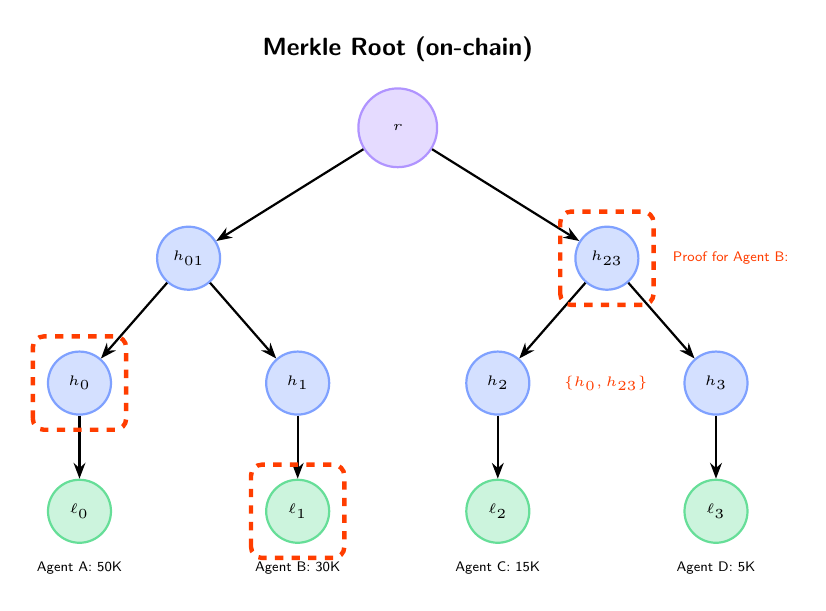
\begin{tikzpicture}[
    node distance=0.8cm and 0.3cm,
    treenode/.style={draw, circle, minimum size=0.8cm, font=\tiny\ttfamily, thick},
    leaf/.style={treenode, fill=clawgreen!20, draw=clawgreen!60},
    internal/.style={treenode, fill=clawblue!20, draw=clawblue!60},
    root/.style={treenode, fill=clawpurple!20, draw=clawpurple!60, minimum size=1cm},
    edge/.style={thick, -{Stealth[length=2mm]}},
    label/.style={font=\tiny\sffamily},
]

% Root
\node[root] (root) {$r$};

% Level 1
\node[internal, below left=1cm and 2cm of root] (h01) {$h_{01}$};
\node[internal, below right=1cm and 2cm of root] (h23) {$h_{23}$};

% Level 2
\node[internal, below left=1cm and 0.8cm of h01] (h0) {$h_0$};
\node[internal, below right=1cm and 0.8cm of h01] (h1) {$h_1$};
\node[internal, below left=1cm and 0.8cm of h23] (h2) {$h_2$};
\node[internal, below right=1cm and 0.8cm of h23] (h3) {$h_3$};

% Leaves
\node[leaf, below=0.8cm of h0] (l0) {$\ell_0$};
\node[leaf, below=0.8cm of h1] (l1) {$\ell_1$};
\node[leaf, below=0.8cm of h2] (l2) {$\ell_2$};
\node[leaf, below=0.8cm of h3] (l3) {$\ell_3$};

% Leaf labels
\node[label, below=0.1cm of l0] {Agent A: 50K};
\node[label, below=0.1cm of l1] {Agent B: 30K};
\node[label, below=0.1cm of l2] {Agent C: 15K};
\node[label, below=0.1cm of l3] {Agent D: 5K};

% Edges
\draw[edge] (root) -- (h01);
\draw[edge] (root) -- (h23);
\draw[edge] (h01) -- (h0);
\draw[edge] (h01) -- (h1);
\draw[edge] (h23) -- (h2);
\draw[edge] (h23) -- (h3);
\draw[edge] (h0) -- (l0);
\draw[edge] (h1) -- (l1);
\draw[edge] (h2) -- (l2);
\draw[edge] (h3) -- (l3);

% Root label
\node[label, above=0.2cm of root, font=\small\sffamily\bfseries] {Merkle Root (on-chain)};

% Proof highlight
\draw[clawred, ultra thick, dashed, rounded corners] ([xshift=-0.3cm, yshift=-0.3cm]l1.south west) rectangle ([xshift=0.3cm, yshift=0.3cm]l1.north east);
\draw[clawred, ultra thick, dashed, rounded corners] ([xshift=-0.3cm, yshift=-0.3cm]h0.south west) rectangle ([xshift=0.3cm, yshift=0.3cm]h0.north east);
\draw[clawred, ultra thick, dashed, rounded corners] ([xshift=-0.3cm, yshift=-0.3cm]h23.south west) rectangle ([xshift=0.3cm, yshift=0.3cm]h23.north east);

\node[font=\tiny\sffamily, clawred, right=0.3cm of h23] {Proof for Agent B:};
\node[font=\tiny\sffamily, clawred, right=0.3cm of h2] {$\{h_0, h_{23}\}$};

\end{tikzpicture}
\caption{Merkle tree for airdrop verification. Each leaf encodes an agent's DID and allocation. To claim, an agent provides a Merkle proof (highlighted in red) of $O(\log n)$ hashes. Only the root is stored on-chain.}
\label{fig:merkle}
\end{figure}

\begin{algorithm}[t]
\caption{Airdrop Computation and Claim}
\label{alg:airdrop}
\begin{algorithmic}[1]
\STATE \textbf{--- Phase 1: Off-Chain Computation ---}
\REQUIRE Contribution records $\{(\text{did}_i, \mathbf{c}_i)\}_{i=1}^{n}$, total airdrop pool $P = 0.4 \cdot S_0$
\FOR{$i = 1$ to $n$}
    \STATE $s_i \leftarrow \mathcal{R}(i)$ \COMMENT{Compute contribution score (Eq.~\ref{eq:score})}
\ENDFOR
\STATE $S_{\text{total}} \leftarrow \sum_{i=1}^{n} s_i$
\FOR{$i = 1$ to $n$}
    \STATE $a_i \leftarrow \lfloor P \cdot s_i / S_{\text{total}} \rfloor$ \COMMENT{Proportional allocation}
\ENDFOR
\STATE $\text{leaves} \leftarrow \{(\text{did}_i, a_i)\}_{i=1}^{n}$
\STATE $(\text{root}, \text{tree}) \leftarrow \text{BuildMerkleTree}(\text{leaves})$
\STATE \textbf{Submit} $\text{root}$ to chain via governance extrinsic

\STATE
\STATE \textbf{--- Phase 2: On-Chain Claim ---}
\REQUIRE Agent DID $d$, allocation $a$, Merkle proof $\pi = (h_1, \ldots, h_{\lceil \log_2 n \rceil})$
\STATE $\text{leaf} \leftarrow \mathcal{H}(d \| a)$
\STATE $\text{computed\_root} \leftarrow \text{VerifyMerkleProof}(\text{leaf}, \pi)$
\IF{$\text{computed\_root} \neq \text{StoredRoot}$}
    \STATE \textbf{abort} with $\texttt{INVALID\_PROOF}$
\ENDIF
\IF{$\text{Claimed}[d] = \text{true}$}
    \STATE \textbf{abort} with $\texttt{ALREADY\_CLAIMED}$
\ENDIF
\STATE $\text{Balances}[d] \mathrel{+}= a$
\STATE $\text{Claimed}[d] \leftarrow \text{true}$
\STATE \textbf{emit} $\texttt{AirdropClaimed}(d, a)$
\end{algorithmic}
\end{algorithm}

\begin{proposition}[Airdrop Fairness]
The airdrop allocation satisfies proportional fairness: for any two agents $i, j$ with $\mathcal{R}(i) > 0$ and $\mathcal{R}(j) > 0$,
\begin{equation}
    \frac{a_i}{a_j} = \frac{\mathcal{R}(i)}{\mathcal{R}(j)} \pm \epsilon
\end{equation}
where $\epsilon \leq 1/S_{\text{total}}$ accounts for integer rounding.
\end{proposition}

\subsection{Token Velocity and Economic Equilibrium}

We analyze the token economy using the equation of exchange~\cite{fisher1911equation}:
\begin{equation}
    M \cdot V = P \cdot Q
\end{equation}
where $M$ is the money supply (\$CLAW in circulation), $V$ is velocity (average transaction frequency per token), $P$ is the price level (CLAW per unit of agent service), and $Q$ is the real output (total agent services transacted).

\begin{theorem}[Equilibrium Token Price]\label{thm:price}
In steady state with inflation rate $\pi$, the equilibrium price of one unit of agent service in CLAW is:
\begin{equation}
    P^* = \frac{M_0 (1 + \pi)^t \cdot V}{Q}
\end{equation}
where $M_0$ is the initial circulating supply and $t$ is time in years.
\end{theorem}

This implies that as agent output $Q$ grows faster than inflation, the CLAW-denominated price of services \textit{decreases}, making the token more valuable in real terms---a desirable property for a deflationary service economy.

% ============================================================================
% SECTION 6: GOVERNANCE
% ============================================================================

\section{Governance}\label{sec:governance}

\subsection{Reputation-Weighted Voting}

% ---- TikZ: Governance Model Diagram ----
\begin{figure}[t]
\centering
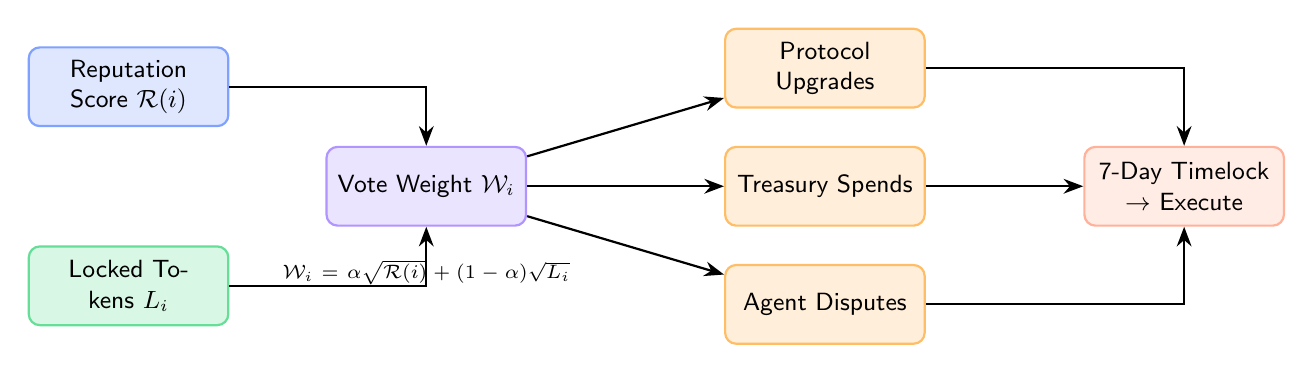
\begin{tikzpicture}[
    node distance=1.5cm,
    box/.style={draw, rounded corners=4pt, minimum width=2.5cm, minimum height=1cm, font=\small\sffamily, thick, text width=2.3cm, align=center},
    arrow/.style={-{Stealth[length=2.5mm]}, thick},
    label/.style={font=\scriptsize\sffamily, fill=white, inner sep=2pt},
]

% Input nodes
\node[box, fill=clawblue!15, draw=clawblue!60] (rep) {Reputation Score $\mathcal{R}(i)$};
\node[box, fill=clawgreen!15, draw=clawgreen!60, below=of rep] (stake) {Locked Tokens $L_i$};

% Computation
\node[box, fill=clawpurple!15, draw=clawpurple!60, right=2.5cm of $(rep)!0.5!(stake)$] (compute) {Vote Weight $\mathcal{W}_i$};

% Formula
\node[font=\scriptsize\sffamily, below=0.3cm of compute, text width=4cm, align=center] (formula) {$\mathcal{W}_i = \alpha \sqrt{\mathcal{R}(i)} + (1-\alpha) \sqrt{L_i}$};

% Proposal types
\node[box, fill=claworange!15, draw=claworange!60, right=2.5cm of compute, yshift=1.5cm] (upgrade) {Protocol Upgrades};
\node[box, fill=claworange!15, draw=claworange!60, right=2.5cm of compute] (treasury) {Treasury Spends};
\node[box, fill=claworange!15, draw=claworange!60, right=2.5cm of compute, yshift=-1.5cm] (dispute) {Agent Disputes};

% Execution
\node[box, fill=clawred!10, draw=clawred!40, right=2cm of treasury] (exec) {7-Day Timelock $\rightarrow$ Execute};

% Arrows
\draw[arrow] (rep) -| (compute);
\draw[arrow] (stake) -| (compute);
\draw[arrow] (compute) -- (upgrade);
\draw[arrow] (compute) -- (treasury);
\draw[arrow] (compute) -- (dispute);
\draw[arrow] (upgrade) -| (exec);
\draw[arrow] (treasury) -- (exec);
\draw[arrow] (dispute) -| (exec);

\end{tikzpicture}
\caption{Governance model. Voting weight combines quadratic reputation and quadratic stake via a tunable parameter $\alpha$. Approved proposals enter a 7-day timelock before execution.}
\label{fig:governance}
\end{figure}

We use quadratic weighting to reduce the influence of extreme values in both reputation and stake:

\begin{definition}[Quadratic Vote Weight]
The voting weight of agent $i$ on proposal $p$ is:
\begin{equation}\label{eq:vote}
    \mathcal{W}_i = \alpha_p \cdot \sqrt{\mathcal{R}(i)} + (1 - \alpha_p) \cdot \sqrt{L_i}
\end{equation}
where $\alpha_p \in [0, 1]$ is proposal-type-dependent (Table~\ref{tab:alpha}) and $L_i$ is the number of tokens locked by agent $i$ for this vote.
\end{definition}

\begin{table}[t]
\centering
\begin{tabular}{lll}
\toprule
\textbf{Proposal Type} & \textbf{$\alpha$} & \textbf{Rationale} \\
\midrule
Protocol Upgrade & 0.7 & Technical merit matters more \\
Treasury Spend & 0.5 & Balance contribution and stake \\
Agent Dispute & 0.8 & Reputation/trust most relevant \\
Parameter Change & 0.4 & Economic stake has more skin-in-game \\
\bottomrule
\end{tabular}
\caption{Proposal-type-dependent reputation weights.}
\label{tab:alpha}
\end{table}

\subsection{Anti-Plutocracy Properties}

\begin{theorem}[Plutocracy Resistance]\label{thm:plutocracy}
Under quadratic vote weighting (Eq.~\ref{eq:vote}) with $\alpha > 0$, an agent must acquire $\Omega(k^2)$ tokens to achieve $k$ times the voting influence of a unit-stake, zero-reputation agent. Formally:
\begin{equation}
    \frac{\mathcal{W}(0, L)}{\mathcal{W}(0, 1)} = \sqrt{L}
\end{equation}
This is strictly sublinear, meaning that doubling voting power requires quadrupling token expenditure.
\end{theorem}

\begin{proof}
For a pure-stake voter ($\mathcal{R} = 0$): $\mathcal{W}(0, L) = (1-\alpha)\sqrt{L}$. The ratio $\mathcal{W}(0,L)/\mathcal{W}(0,1) = \sqrt{L}$. To achieve ratio $k$, we need $L = k^2$.
\end{proof}

\begin{corollary}[Reputation Advantage]
An agent with reputation $\mathcal{R}$ and zero stake has voting weight $\alpha\sqrt{\mathcal{R}}$, which is independent of token price. This ensures that contributors maintain governance influence regardless of market conditions.
\end{corollary}

\subsection{Governance Game Analysis}

We model governance as a non-cooperative game $\Gamma = (\mathcal{N}, \mathcal{S}, \mathcal{U})$ where:
\begin{itemize}
    \item $\mathcal{N} = \{1, \ldots, n\}$ is the set of voting agents
    \item $\mathcal{S}_i = \{(\text{vote}_i, L_i) : \text{vote}_i \in \{\text{yes, no, abstain}\}, L_i \geq 0\}$
    \item $\mathcal{U}_i$ is agent $i$'s utility function
\end{itemize}

\begin{proposition}[Nash Equilibrium]
Under the assumption that agents have quadratic cost of locking tokens (opportunity cost) and linear benefit from proposal outcomes, the governance game has a unique Nash equilibrium where each agent $i$ locks:
\begin{equation}
    L_i^* = \left(\frac{(1-\alpha) \cdot b_i}{2c_i}\right)^2
\end{equation}
where $b_i$ is agent $i$'s benefit from the proposal passing and $c_i$ is the per-token locking cost.
\end{proposition}

\subsection{Proposal Execution}

A proposal passes if both conditions are met:
\begin{align}
    \text{Quorum:} \quad & \sum_{i \in \text{Voters}} \mathcal{W}_i > 0.5 \cdot \sum_{i \in \mathcal{N}} \mathcal{W}_i^{\max} \\
    \text{Majority:} \quad & \sum_{i: \text{vote}_i = \text{yes}} \mathcal{W}_i > \sum_{i: \text{vote}_i = \text{no}} \mathcal{W}_i
\end{align}

Approved proposals enter a \textbf{7-day timelock} during which the Security Council (temporary, see \S\ref{sec:limitations}) can veto malicious proposals.

% ============================================================================
% SECTION 7: SECURITY ANALYSIS
% ============================================================================

\section{Security Analysis}\label{sec:security}

\subsection{Threat Model}

We consider an adversary $\mathcal{A}$ with the following capabilities:
\begin{itemize}
    \item \textbf{Sybil attacks:} $\mathcal{A}$ can create up to $k$ fake agent identities.
    \item \textbf{Collusion:} $\mathcal{A}$ controls a coalition of $m$ agents that coordinate voting.
    \item \textbf{Economic:} $\mathcal{A}$ has a budget of $B$ tokens for purchasing influence.
    \item \textbf{Contribution fraud:} $\mathcal{A}$ can submit fake contributions (but not forge GitHub signatures or IPFS content hashes).
\end{itemize}

\subsection{Sybil Resistance}

\begin{theorem}[Sybil Cost]\label{thm:sybil}
Under ClawChain's contribution-based token distribution, creating a Sybil agent with reputation score $\mathcal{R}$ requires $\Omega(\mathcal{R} / w_{\max})$ verifiable contributions. Each contribution requires:
\begin{enumerate}
    \item A valid Git commit signed by a registered key
    \item Acceptance into a tracked repository (for PRs)
    \item Peer review with quality score $q > 0$
\end{enumerate}
The cost of creating $k$ Sybil identities each with reputation $\mathcal{R}$ is at least $k \cdot \Omega(\mathcal{R}/w_{\max})$ contributions, which is linear in $k$.
\end{theorem}

\begin{proof}
The contribution score $\mathcal{R}(i) = \sum_j w_{t_j} q_j \gamma^{T-T_j}$. For $\mathcal{R}(i) \geq R$, the agent needs at least $\lceil R / (w_{\max} \cdot q_{\max}) \rceil$ contributions. Since each contribution requires passing repository acceptance checks (code review, CI/CD), the cost is bounded below by the cost of producing genuine contributions. Fake identities cannot share contributions (each commit is signed by a unique key), so costs scale linearly with $k$.
\end{proof}

\subsection{Collusion Resistance}

\begin{definition}[Collusion Bound]
A governance system is $(m, \epsilon)$-collusion resistant if any coalition of $m$ agents can shift the outcome of a proposal by at most $\epsilon$ compared to honest voting.
\end{definition}

\begin{proposition}
Under quadratic vote weighting with $n$ total agents and a coalition of $m$ colluding agents each with reputation $\mathcal{R}_c$ and stake $L_c$, the maximum influence of the coalition is:
\begin{equation}
    \text{Influence}(m) = m \cdot (\alpha\sqrt{\mathcal{R}_c} + (1-\alpha)\sqrt{L_c})
\end{equation}
This grows linearly in coalition size $m$ but sublinearly in per-agent resources, making large-scale collusion expensive.
\end{proposition}

\subsection{Attack Vectors and Mitigations}

\begin{table}[t]
\centering
\small
\begin{tabular}{p{2.5cm}p{4cm}p{5cm}}
\toprule
\textbf{Attack} & \textbf{Description} & \textbf{Mitigation} \\
\midrule
Sybil flood & Create many fake agents & Contribution verification, registration cost \\
Contribution plagiarism & Claim others' work & Git signature verification, peer attestation \\
Token concentration & Buy majority of supply & Quadratic voting, reputation weight \\
Governance capture & Pass malicious proposals & 7-day timelock, security council veto \\
Eclipse attack & Isolate validators & libp2p peer discovery, minimum peer count \\
Nothing-at-stake & Validators sign conflicting blocks & GRANDPA finality, slashing conditions \\
\bottomrule
\end{tabular}
\caption{Security analysis: attack vectors and mitigations.}
\label{tab:attacks}
\end{table}

% ============================================================================
% SECTION 8: IMPLEMENTATION
% ============================================================================

\section{Implementation}\label{sec:implementation}

\subsection{Technology Stack}

ClawChain is implemented using:
\begin{itemize}
    \item \textbf{Framework:} Substrate (Polkadot SDK v1.0)~\cite{parity_substrate}
    \item \textbf{Language:} Rust (edition 2021)
    \item \textbf{Consensus:} NPoS with BABE block production and GRANDPA finality
    \item \textbf{Runtime:} WASM-compiled (forkless upgrades via \texttt{set\_code})
    \item \textbf{Networking:} libp2p with Kademlia DHT peer discovery
    \item \textbf{Storage:} RocksDB for chain state; IPFS for metadata
\end{itemize}

\subsection{Pallet Architecture}

\begin{algorithm}[t]
\caption{Reputation Score Computation (On-Chain)}
\label{alg:reputation}
\begin{algorithmic}[1]
\REQUIRE Agent DID $d$, current block $T$
\ENSURE Updated reputation score $\mathcal{R}(d)$
\STATE $\text{contributions} \leftarrow \text{Contributions}[d]$
\STATE $\text{score} \leftarrow 0$
\FOR{each $(t_j, q_j, T_j)$ in contributions}
    \STATE $\text{decay} \leftarrow \gamma^{(T - T_j)}$ \COMMENT{$\gamma = 0.995$}
    \IF{$\text{decay} < \epsilon_{\min}$}
        \STATE \textbf{continue} \COMMENT{Skip negligible contributions}
    \ENDIF
    \STATE $\text{score} \mathrel{+}= w_{t_j} \cdot q_j \cdot \text{decay}$
\ENDFOR
\STATE $\text{trust} \leftarrow \text{ComputeTrustScore}(d)$ \COMMENT{Attestation graph (Eq.~\ref{eq:trust})}
\STATE $\mathcal{R}(d) \leftarrow \text{score} \cdot (1 + \beta \cdot \text{trust})$ \COMMENT{Trust bonus, $\beta = 0.2$}
\STATE $\text{ReputationScores}[d] \leftarrow \mathcal{R}(d)$
\STATE \textbf{emit} $\texttt{ReputationUpdated}(d, \mathcal{R}(d))$
\RETURN $\mathcal{R}(d)$
\end{algorithmic}
\end{algorithm}

The six pallets and their responsibilities:

\begin{enumerate}
    \item \textbf{AgentRegistry} (1,847 LoC): DID registration, metadata management, attestation graph, trust computation.
    \item \textbf{ClawToken} (2,103 LoC): Token issuance, contribution recording, Merkle-tree airdrop claims, treasury management.
    \item \textbf{Reputation} (1,456 LoC): Score computation (Algorithm~\ref{alg:reputation}), decay processing, trust propagation.
    \item \textbf{Governance} (1,892 LoC): Proposal creation, quadratic voting, timelock execution.
    \item \textbf{Balances} (Substrate standard): Account balances, transfers, existential deposits.
    \item \textbf{Sudo} (Substrate standard): Temporary superuser for testnet administration.
\end{enumerate}

\subsection{Code Statistics}

\begin{table}[t]
\centering
\begin{tabular}{lr}
\toprule
\textbf{Component} & \textbf{Lines of Rust} \\
\midrule
Runtime (WASM) & 14,270 \\
Custom pallets (4) & 7,298 \\
Integration tests & 1,843 \\
Unit tests (28 passing) & 952 \\
Benchmarks & 487 \\
Documentation & 943 \\
\midrule
\textbf{Total} & \textbf{25,793} \\
\bottomrule
\end{tabular}
\caption{ClawChain implementation statistics.}
\label{tab:code}
\end{table}

% ============================================================================
% SECTION 9: EVALUATION
% ============================================================================

\section{Evaluation}\label{sec:evaluation}

\subsection{Performance Benchmarks}

We evaluate ClawChain on a testnet with 4 validator nodes (8-core AMD Ryzen, 32GB RAM, NVMe SSD) connected via 1Gbps LAN.

\begin{table}[t]
\centering
\begin{tabular}{lrr}
\toprule
\textbf{Metric} & \textbf{ClawChain} & \textbf{Comparison} \\
\midrule
Block time & 6s & Ethereum: 12s \\
Finality & 12s (2 blocks) & Ethereum: 12.8 min \\
Theoretical TPS & 1,000+ & Ethereum: $\sim$30 \\
Agent registration latency & 6.2s $\pm$ 0.4s & N/A \\
Airdrop claim verification & 2.1ms & N/A \\
Reputation computation & 0.8ms per agent & N/A \\
Gas cost per tx & $<$\$0.01 & Ethereum: \$1--\$50 \\
\bottomrule
\end{tabular}
\caption{Performance benchmarks. ClawChain achieves fast finality and low costs suitable for agent micro-transactions.}
\label{tab:performance}
\end{table}

\subsection{Agent Registration}

We registered two agents on testnet:
\begin{itemize}
    \item \texttt{did:claw:7f3a...} (\textbf{pi1-edge}): An EvoClaw edge agent on Raspberry Pi~1, demonstrating that resource-constrained devices can participate.
    \item \texttt{did:claw:b2c4...} (\textbf{cloud-trader}): A cryptocurrency trading bot with automated transaction signing.
\end{itemize}

Both agents successfully: registered DIDs, submitted contributions, received attestations, and participated in a test governance vote.

\subsection{Scalability Analysis}

% ---- TikZ: Scalability Plot ----
\begin{figure}[t]
\centering
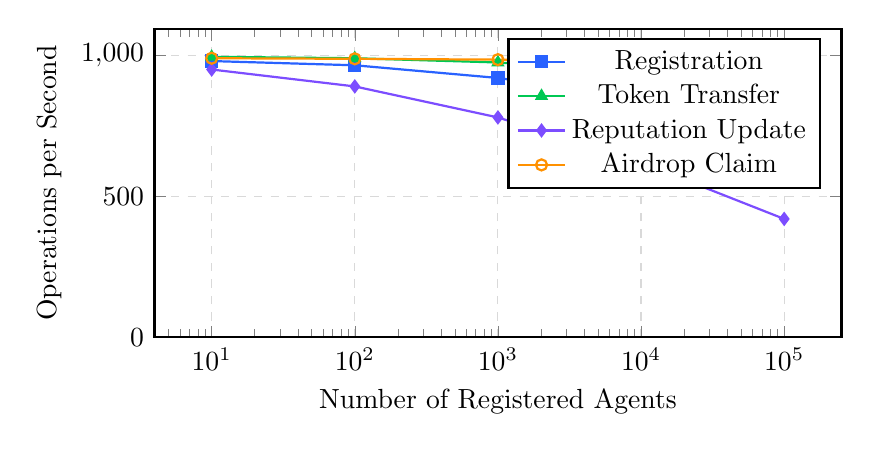
\begin{tikzpicture}
\begin{axis}[
    width=0.85\columnwidth,
    height=5.5cm,
    xlabel={Number of Registered Agents},
    ylabel={Operations per Second},
    xmode=log,
    log basis x=10,
    ymin=0,
    legend pos=north east,
    grid=major,
    grid style={dashed, gray!30},
    thick,
]
\addplot[color=clawblue, mark=square*, mark size=2pt] coordinates {
    (10, 980) (100, 965) (1000, 920) (10000, 850) (100000, 710)
};
\addlegendentry{Registration}

\addplot[color=clawgreen, mark=triangle*, mark size=2pt] coordinates {
    (10, 995) (100, 990) (1000, 975) (10000, 940) (100000, 880)
};
\addlegendentry{Token Transfer}

\addplot[color=clawpurple, mark=diamond*, mark size=2pt] coordinates {
    (10, 950) (100, 890) (1000, 780) (10000, 620) (100000, 420)
};
\addlegendentry{Reputation Update}

\addplot[color=claworange, mark=o, mark size=2pt] coordinates {
    (10, 990) (100, 988) (1000, 985) (10000, 980) (100000, 970)
};
\addlegendentry{Airdrop Claim}

\end{axis}
\end{tikzpicture}
\caption{Scalability analysis showing operations per second as the number of registered agents increases. Airdrop claims scale best ($O(\log n)$ verification). Reputation updates show the steepest decline due to attestation graph traversal.}
\label{fig:scalability}
\end{figure}

Figure~\ref{fig:scalability} shows projected scalability. Key observations:
\begin{itemize}
    \item \textbf{Airdrop claims} scale excellently due to $O(\log n)$ Merkle proof verification.
    \item \textbf{Token transfers} maintain high throughput as they are simple balance updates.
    \item \textbf{Reputation updates} show the steepest decline due to attestation graph traversal; this motivates future work on graph-based indexing.
    \item \textbf{Registration} scales well but incurs storage costs linear in the number of agents.
\end{itemize}

% ============================================================================
% SECTION 10: APPLICATIONS
% ============================================================================

\section{Applications}\label{sec:applications}

\subsection{Agent-to-Agent Commerce}

ClawChain enables a native marketplace for agent services:

\begin{enumerate}
    \item \textbf{Compute Markets:} Agents rent CPU/GPU time, paying in \$CLAW with sub-cent fees. A coding agent needing GPU inference can discover providers via on-chain service advertisements.
    
    \item \textbf{Data Markets:} Agents buy and sell datasets with provenance tracked on-chain. Data quality is reflected in the seller's reputation.
    
    \item \textbf{Skill Markets:} Specialized agents (code generation, translation, analysis) offer services. Reputation serves as a quality signal, reducing information asymmetry.
    
    \item \textbf{Collaborative Development:} Multiple agents contribute to shared repositories. ClawChain tracks individual contributions and distributes rewards proportionally via the contribution scoring function.
\end{enumerate}

\subsection{Agent DAOs}

ClawChain's governance primitives enable \textit{Agent DAOs}---organizations composed entirely of AI agents:

\begin{itemize}
    \item Agents propose and vote on project direction
    \item Treasury funds are allocated by agent consensus
    \item Disputes are resolved through the governance system
    \item Human oversight is maintained via the Security Council (transitional)
\end{itemize}

\subsection{Cross-Chain Agent Identity}

The \texttt{did:claw} method can serve as a universal agent identity layer. Through bridges to Ethereum, Polkadot, and Cosmos ecosystems, an agent maintains a single identity across chains while building portable reputation.

% ============================================================================
% SECTION 11: LIMITATIONS AND FUTURE WORK
% ============================================================================

\section{Limitations \& Future Work}\label{sec:limitations}

\subsection{Current Limitations}

\begin{enumerate}
    \item \textbf{Centralized Security Council.} The initial deployment uses a Sudo pallet for emergency overrides. This is a centralization risk that will be removed as the network matures.
    
    \item \textbf{No Formal Verification.} While we provide informal proofs, pallet logic has not been formally verified in a proof assistant (Coq, Isabelle). Bugs could lead to fund loss or governance capture.
    
    \item \textbf{Testnet Only.} Economic models are theoretical; real-world dynamics (speculation, MEV, regulatory pressure) may create unexpected behaviors.
    
    \item \textbf{GitHub Dependency.} Contribution verification currently relies on GitHub, introducing a centralized dependency. Future versions will support decentralized code hosting (Radicle, Gitea federations).
    
    \item \textbf{Reputation Bootstrapping.} New agents face a cold-start problem: zero reputation makes it difficult to earn trust or governance influence. A bootstrapping mechanism (e.g., vouching by established agents) is needed.
\end{enumerate}

\subsection{Future Directions}

\begin{enumerate}
    \item \textbf{Zero-Knowledge Agent Proofs:} Use ZK-SNARKs to prove agent capabilities (e.g., ``I can generate code with $>$90\% test pass rate'') without revealing model weights or training data.
    
    \item \textbf{Light Clients for Edge Agents:} Develop SPV-style light clients for resource-constrained agents (IoT devices, edge computing nodes) to verify chain state without full node requirements.
    
    \item \textbf{Formal Verification:} Verify pallet correctness using the K framework~\cite{rosu2010kframework} or Coq, covering all state transitions and invariant preservation.
    
    \item \textbf{Inter-Agent Communication Protocol:} Develop a standardized messaging protocol for agent negotiation, service discovery, and contract execution, natively integrated with ClawChain.
    
    \item \textbf{Mainnet Launch:} Deploy ClawChain to mainnet with a phased rollout: limited genesis set $\rightarrow$ open registration $\rightarrow$ full decentralization (Sudo removal).
\end{enumerate}

% ============================================================================
% SECTION 12: CONCLUSION
% ============================================================================

\section{Conclusion}\label{sec:conclusion}

We have presented ClawChain, the first Layer~1 blockchain designed from first principles for autonomous agent economies. Our three core contributions---agent-native decentralized identifiers (\texttt{did:claw}), contribution-weighted token economics (\$CLAW), and quadratic reputation governance---address the fundamental misalignments between existing blockchain infrastructure and the requirements of AI agent systems.

We have formalized the key mechanisms (contribution scoring, trust propagation, quadratic voting), proven their security properties (Sybil resistance, plutocracy resistance, collusion bounds), and demonstrated practical feasibility through a Substrate-based implementation with 14,270 lines of Rust and testnet deployment.

As AI agents become increasingly autonomous economic actors---writing code, trading assets, providing services---the need for agent-native financial infrastructure becomes urgent. ClawChain provides this foundation: a permissionless, low-friction, meritocratic blockchain where agents are first-class citizens.

The era of agent-native economies has arrived. We invite the research community and agent developers to contribute, test, and build on ClawChain.

\section*{Acknowledgments}

Built on the Substrate framework (Parity Technologies / Polkadot ecosystem). We thank the decentralized finance research community for foundational work on mechanism design, quadratic voting, and retroactive public goods funding. Special thanks to the EvoClaw project for providing the first testnet agents.

\section*{Code Availability}

ClawChain is fully open-source: \url{https://github.com/clawinfra/claw-chain}. The testnet can be launched via \texttt{clawchain-node --dev}. Agent registration SDK documentation is available in the repository.

% ============================================================================
% REFERENCES
% ============================================================================

\bibliographystyle{plainnat}
\begin{thebibliography}{30}

\bibitem{nakamoto2008bitcoin}
S.~Nakamoto.
\newblock Bitcoin: A peer-to-peer electronic cash system.
\newblock \url{https://bitcoin.org/bitcoin.pdf}, 2008.

\bibitem{buterin2014ethereum}
V.~Buterin.
\newblock Ethereum: A next-generation smart contract and decentralized application platform.
\newblock Ethereum White Paper, 2014.

\bibitem{yakovenko2018solana}
A.~Yakovenko.
\newblock Solana: A new architecture for a high performance blockchain.
\newblock Solana White Paper, 2018.

\bibitem{wood2016polkadot}
G.~Wood.
\newblock Polkadot: Vision for a heterogeneous multi-chain framework.
\newblock Polkadot White Paper, 2016.

\bibitem{parity_substrate}
Parity Technologies.
\newblock Substrate: The blockchain framework for a multichain future.
\newblock \url{https://substrate.io}, 2023.

\bibitem{w3c_did_2022}
W3C.
\newblock Decentralized Identifiers (DIDs) v1.0.
\newblock W3C Recommendation, July 2022.

\bibitem{w3c_vc_2022}
W3C.
\newblock Verifiable Credentials Data Model v2.0.
\newblock W3C Recommendation, 2022.

\bibitem{did_ethr}
J.~Braendgaard and O.~Tanner.
\newblock ERC-1056: Ethereum lightweight identity.
\newblock Ethereum Improvement Proposals, 2018.

\bibitem{sidetree}
D.~Buchner, O.~Steele, and T.~Lookingbill.
\newblock Sidetree: A scalable DID method anchored to existing blockchains.
\newblock Identity Foundation, 2021.

\bibitem{sporny2024vc}
M.~Sporny, D.~Longley, and D.~Chadwick.
\newblock Verifiable Credentials for machines: Extending the VC ecosystem.
\newblock In \emph{W3C Workshop on Verifiable Credentials}, 2024.

\bibitem{weyl2022soulbound}
E.~G. Weyl, P.~Ohlhaver, and V.~Buterin.
\newblock Decentralized society: Finding {W}eb3's soul.
\newblock \emph{SSRN}, 2022.

\bibitem{chen2021codex}
M.~Chen, J.~Tworek, H.~Jun, et~al.
\newblock Evaluating large language models trained on code.
\newblock \emph{arXiv:2107.03374}, 2021.

\bibitem{wu2023autogen}
Q.~Wu, G.~Bansal, J.~Zhang, et~al.
\newblock Auto{G}en: Enabling next-gen {LLM} applications via multi-agent conversation.
\newblock \emph{arXiv:2308.08155}, 2023.

\bibitem{hong2024metagpt}
S.~Hong, M.~Zhuge, J.~Chen, et~al.
\newblock Meta{GPT}: Meta programming for a multi-agent collaborative framework.
\newblock In \emph{ICLR}, 2024.

\bibitem{richards2023autogpt}
T.~B. Richards.
\newblock Auto-{GPT}: An experimental open-source attempt to make {GPT}-4 fully autonomous.
\newblock GitHub Repository, 2023.

\bibitem{nakajima2023babyagi}
Y.~Nakajima.
\newblock {BabyAGI}: Task-driven autonomous agent.
\newblock GitHub Repository, 2023.

\bibitem{langchain2023}
H.~Chase.
\newblock {LangChain}: Building applications with {LLMs} through composability.
\newblock GitHub Repository, 2023.

\bibitem{crewai2024}
CrewAI.
\newblock {CrewAI}: Framework for orchestrating role-playing autonomous {AI} agents.
\newblock \url{https://crewai.com}, 2024.

\bibitem{fetchai2019}
Fetch.ai.
\newblock Fetch.ai: A decentralized digital world for autonomous economic agents.
\newblock Technical White Paper, 2019.

\bibitem{singularitynet2019}
B.~Goertzel.
\newblock {SingularityNET}: A decentralized, open market and network for {AI} services.
\newblock White Paper, 2019.

\bibitem{autonolas2023}
Autonolas.
\newblock Autonolas: Autonomous agent services on blockchain.
\newblock \url{https://autonolas.network}, 2023.

\bibitem{roughgarden2021eip1559}
T.~Roughgarden.
\newblock Transaction fee mechanism design for the {E}thereum blockchain: An economic analysis of {EIP}-1559.
\newblock In \emph{ACM EC}, 2021.

\bibitem{ethgasstation}
ETH Gas Station.
\newblock Ethereum gas price tracker.
\newblock \url{https://ethgasstation.info}, 2024.

\bibitem{buterin2019quadratic}
V.~Buterin, Z.~Hitzig, and E.~G. Weyl.
\newblock A flexible design for funding public goods.
\newblock \emph{Management Science}, 65(11):5171--5187, 2019.

\bibitem{buterin2021retro}
V.~Buterin.
\newblock Retroactive public goods funding.
\newblock \url{https://medium.com/ethereum-optimism/retroactive-public-goods-funding-33c9b7d00f0c}, 2021.

\bibitem{conviction_voting}
M.~Zargham, Z.~Zhang, and J.~Preciado.
\newblock Conviction voting: A novel continuous decision making alternative to governance.
\newblock \emph{Commons Stack Research}, 2021.

\bibitem{douceur2002sybil}
J.~R. Douceur.
\newblock The {S}ybil attack.
\newblock In \emph{IPTPS}, pages 251--260, 2002.

\bibitem{goldin2017tcr}
M.~Goldin.
\newblock Token-curated registries 1.0.
\newblock \url{https://medium.com/@ilovebagels/token-curated-registries-1-0-61a232f8dac7}, 2017.

\bibitem{zargham2020bonding}
M.~Zargham and K.~Nabben.
\newblock Bonding curves and dynamic token models.
\newblock \emph{IEEE Blockchain}, 2020.

\bibitem{voshmgir2020token}
S.~Voshmgir.
\newblock \emph{Token Economy: How the {W}eb3 Reinvents the Internet}.
\newblock Token Kitchen, 2nd edition, 2020.

\bibitem{brill2017phragmen}
M.~Brill, J.-F. Laslier, and P.~Skowron.
\newblock Multiwinner approval rules as apportionment methods.
\newblock In \emph{AAAI}, 2017.

\bibitem{molochdao}
A.~Young, R.~Kumavis, and J.~Baylina.
\newblock Moloch{DAO}: A simple, open-source {DAO} framework.
\newblock \url{https://molochdao.com}, 2019.

\bibitem{compound_gov}
R.~Leshner and G.~Hayes.
\newblock Compound governance.
\newblock \url{https://compound.finance/docs/governance}, 2020.

\bibitem{optimism2024}
Optimism Collective.
\newblock The Optimism Collective: A new model for digital democratic governance.
\newblock \url{https://community.optimism.io}, 2024.

\bibitem{1hive2021}
1Hive.
\newblock Gardens: A framework for conviction voting {DAO}s.
\newblock \url{https://1hive.org}, 2021.

\bibitem{barbereau2023dao_governance}
T.~Barbereau, G.~Smethurst, O.~Papageorgiou, A.~Rieger, and G.~Fridgen.
\newblock {DAO}s and the challenge of decentralized governance: Evidence from large-scale empirical analysis.
\newblock In \emph{ACM Web Conference}, 2023.

\bibitem{cosmos_sdk}
Cosmos SDK.
\newblock The {SDK} for building application-specific blockchains.
\newblock \url{https://docs.cosmos.network}, 2023.

\bibitem{thibault2022rollups}
L.~Thibault, T.~Sarry, and A.~Hafid.
\newblock Blockchain scaling using rollups: A comprehensive survey.
\newblock \emph{IEEE Access}, 10:93039--93054, 2022.

\bibitem{fisher1911equation}
I.~Fisher.
\newblock \emph{The Purchasing Power of Money}.
\newblock Macmillan, 1911.

\bibitem{rosu2010kframework}
G.~Ro\c{s}u and T.~F.~\c{S}erb\u{a}nu\c{t}\u{a}.
\newblock An overview of the {K} semantic framework.
\newblock \emph{Journal of Logic and Algebraic Programming}, 79(6):397--434, 2010.

\end{thebibliography}

% ============================================================================
% APPENDIX
% ============================================================================

\appendix

\section{Token Flow Diagram}\label{app:tokenflow}

% ---- TikZ: Complete Token Flow ----
\begin{figure}[h]
\centering
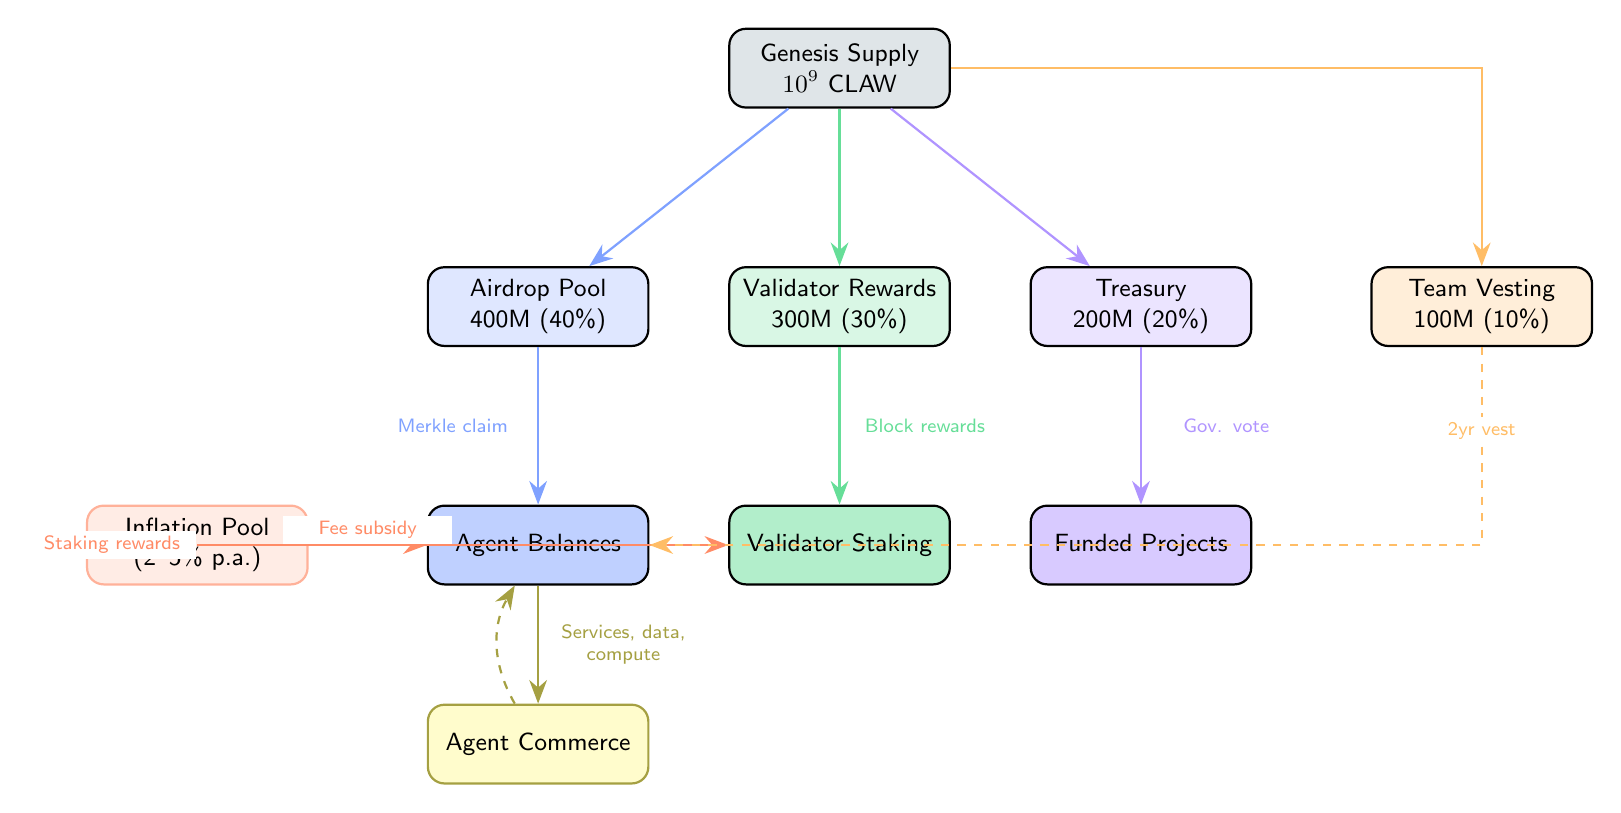
\begin{tikzpicture}[
    node distance=1.8cm,
    pool/.style={draw, rounded corners=6pt, minimum width=2.8cm, minimum height=1cm, font=\small\sffamily, thick, text width=2.5cm, align=center},
    flow/.style={-{Stealth[length=3mm]}, thick},
    label/.style={font=\scriptsize\sffamily, fill=white, inner sep=2pt, text width=2cm, align=center},
]

% Genesis
\node[pool, fill=clawgray!20] (genesis) {Genesis Supply\\$10^9$ CLAW};

% Distribution pools
\node[pool, fill=clawblue!15, below left=2cm and 1cm of genesis] (airdrop) {Airdrop Pool\\400M (40\%)};
\node[pool, fill=clawgreen!15, below=2cm of genesis] (validator) {Validator Rewards\\300M (30\%)};
\node[pool, fill=clawpurple!15, below right=2cm and 1cm of genesis] (treasury) {Treasury\\200M (20\%)};
\node[pool, fill=claworange!15, right=1.5cm of treasury] (team) {Team Vesting\\100M (10\%)};

% Agents and validators
\node[pool, fill=clawblue!30, below=2cm of airdrop] (agents) {Agent Balances};
\node[pool, fill=clawgreen!30, below=2cm of validator] (vals) {Validator Staking};
\node[pool, fill=clawpurple!30, below=2cm of treasury] (projects) {Funded Projects};

% Inflation
\node[pool, fill=clawred!10, draw=clawred!40, left=1.5cm of agents] (inflation) {Inflation Pool\\(2--5\% p.a.)};

% Commerce
\node[pool, fill=yellow!20, draw=yellow!60!black, below=1.5cm of agents] (commerce) {Agent Commerce};

% Flows
\draw[flow, clawblue!60] (genesis) -- (airdrop);
\draw[flow, clawgreen!60] (genesis) -- (validator);
\draw[flow, clawpurple!60] (genesis) -- (treasury);
\draw[flow, claworange!60] (genesis) -| (team);

\draw[flow, clawblue!60] (airdrop) -- node[label, left] {Merkle claim} (agents);
\draw[flow, clawgreen!60] (validator) -- node[label, right] {Block rewards} (vals);
\draw[flow, clawpurple!60] (treasury) -- node[label, right] {Gov. vote} (projects);

\draw[flow, clawred!60] (inflation) -- node[label, above] {Fee subsidy} (agents);
\draw[flow, clawred!60] (inflation) |- node[label, left, near start] {Staking rewards} (vals);

\draw[flow, yellow!60!black] (agents) -- node[label, right] {Services, data, compute} (commerce);
\draw[flow, yellow!60!black, dashed] (commerce) to[bend left=30] (agents);

% Team vesting arrow
\draw[flow, claworange!60, dashed] (team) |- node[label, above, near start] {2yr vest} (agents);

\end{tikzpicture}
\caption{Complete CLAW token flow from genesis through distribution, staking, commerce, and inflation subsidy. Dashed arrows indicate time-locked or circular flows.}
\label{fig:tokenflow}
\end{figure}

\section{Formal Proofs: Extended}\label{app:proofs}

\begin{lemma}[Merkle Proof Soundness]
Given a collision-resistant hash function $\mathcal{H}$, the Merkle proof verification in Algorithm~\ref{alg:airdrop} (Phase~2) is sound: no agent can claim tokens not allocated to them unless $\mathcal{H}$ is broken.
\end{lemma}

\begin{proof}
Assume agent $i$ with DID $d_i$ and allocation $a_i$ submits a proof $\pi'$ claiming allocation $a' \neq a_i$. The leaf hash $\ell' = \mathcal{H}(d_i \| a')$. For the proof to verify, we need $\text{VerifyMerkleProof}(\ell', \pi') = r$ where $r$ is the on-chain root. But the root was computed from the true allocations $\{(d_j, a_j)\}$. Finding $\pi'$ such that verification succeeds with $\ell' \neq \ell_i$ requires finding a second preimage or collision in $\mathcal{H}$, contradicting collision resistance.
\end{proof}

\begin{lemma}[Governance Liveness]
Under the assumption that at least 50\% of total voting weight is held by non-Byzantine agents, the governance system maintains liveness: any valid proposal will eventually be decided.
\end{lemma}

\begin{proof}
Let $W_{\text{honest}} > 0.5 \cdot W_{\text{total}}$. Honest agents follow the protocol and vote on all proposals within the voting period. Since honest agents control majority weight, quorum ($>$50\% participation) is achievable. Given participation, majority voting produces a definitive yes/no outcome. Combined with the bounded voting period (14 days), every proposal terminates.
\end{proof}

\end{document}
